
\documentclass[modern]{aastex62}
%linenumbers

%\documentclass[DM,authoryear,toc]{lsstdoc}
\newcommand{\docRef}{set the Reference with {$\backslash$}setDocRef}
\newcommand{\setDocRef}[1]{
   \renewcommand{\docRef}{#1}
}

\setDocRef{DMTN-115}
\usepackage{newtxtext,newtxmath} % this is causing the etoolbox warning
\usepackage[USenglish]{babel}
\usepackage[utf8]{inputenc}
\usepackage[T1]{fontenc}
\usepackage{comment}
\usepackage{enumitem}
\usepackage{glossaries}
\usepackage{todonotes}
\usepackage{collect}
\usepackage{wrapfig}

\setlist{noitemsep}

\graphicspath{{./}{./figures/}{./images}}



% Add your own macros here:

\newcommand{\Comment}[3]{\textcolor{#1}{(#2: #3)}}
\newcommand{\AMS}[1]{\Comment{red}{AMS}{#1}} % Arfon Smith's comments

% lsstdoc documentation: https://lsst-texmf.lsst.io/lsstdoc.html

\providecommand{\secref}[1]{Section~\ref{#1}}
\providecommand{\appref}[1]{Appendix~\ref{#1}}
\providecommand{\tabref}[1]{Table~\ref{#1}}
\providecommand{\figref}[1]{Figure~\ref{#1}}
\providecommand{\eqnref}[1]{Eq.~\ref{#1}}
\providecommand{\recref}[1]{REC-\ref{#1}}




\begin{document}



\author{William~O'Mullane.}
\affiliation{Large Synoptic Survey Telescope (LSST/AURA)}
\author{Niall~Gaffney}
\affiliation{Texas Advanced Computing Center}
\author{Frossie~Economou}
\affiliation{Large Synoptic Survey Telescope (LSST/AURA)}
\author{Arfon~M.~Smith}
\affiliation{Space Telescope Science Institute}
\author{J.~Ross~Thomson}
\affiliation{Google}
\author{Tim~Jenness}
\affiliation{Large Synoptic Survey Telescope (LSST/AURA)}

\date{\today}

\keywords{Astronomy, Astrophysics, Data Management, Computing, HPC, HTC, Networking, Cloud, Files   }
%should be 350 chars
\begin{abstract}
Many astronomy data centres still work on filesystems.
Industry has moved on;  current practice in  computing infrastructure is to achieve Big Data scalability using  object stores rather than Posix file systems. This presents us with  opportunities  for portability and reuse of software underlying processing and archive  systems  but it also causes problems for legacy implementations in current data centers.

\end{abstract}


% Create the title page.
\title{The demise of the filesystem}
%\maketitle
 \hypersetup{pdftitle={\@title}, pdfauthor={\@author}, pdfkeywords={\docRef \@keywords}}

\section{Introduction} \label{sec:intro}

{\bf Executive summary:} the filesystem notion limits our ability to scale processing and has long since been dropped by industry. Astronomy needs to move on.

Object Stores are nothing new to Astronomy.  \gls{FITS} and \gls{IRAF} tapes are examples
of object stores that were used when file systems were unable to handle the volumes
of data being produced. Even then, standards for migrating from \gls{Object} Store to file
systems were created, allowing for objects to be retrieved into a predefined namespace
on disk.  The explosion of individual \gls{POSIX} disk capacity and \gls{POSIX}-like file systems
have produced generations of researchers who have never used an \gls{Object} Store. While
this growth has supported data systems up till now, the size and complexity of
data being produced by surveys and even pointed telescope archives is reaching
scales where the requirements placed on file access by the \gls{POSIX} standard are
significantly hindering our ability to work with data.  Different parallel file systems
have different strengths and weaknesses.

At large scale, data service providers such as Dropbox and \gls{AWS} do not store files
in \gls{POSIX} systems.  Rather they present the illusion of directory structure layered over
large scale object stores. This allows for faster file access, with only \gls{CRUD} style
functions taking place on each object.  Further, as the pseudo-filesystem layer is simply a
view of structure typically provided by a graph database, users can arrange or potentially
have real time query driven structure for the file organization, removing how many now
organize data through a sea of nested symlinks.
Some provide local \gls{POSIX} caches of that users view of the
pseudo-filesystem, allowing for \gls{POSIX} style applications to access the files with
fopen, fscan, and fclose standard commands. Additionally, these providers do
not show users how data are stored. One can simply request data in the format
needed (e.g. Excel, \gls{CSV}, or as I assume it is the \gls{JSON} format the web apps
use for sheets).   At scale, applications often forgo
such Posix layers and simply use the \gls{CRUD} interfaces to the objects to load them into
memory, act on the objects, and then update or delete them, in the format they need
as input and with the format they naively produce. Further, the data providers need
not update their data archive when formats change, simply provide a new updated
data access format that can be fueled by legacy data formats.

It is time for Astronomy data researchers to follow this curve. As users have migrated
from using tools on their laptops to support collaboration while reducing
individuals need to manage their systems (Jupyter Hubs, Overleaf, Google Slides),
so should astronomical data processing and analysis. We propose the adoption of
a common Astronomical data access \gls{API} layer.


\section{Recommendation }
We need to adopt an industry  standard layered architecture for astronomy processing and data access as
depicted in \figref{fig:ci}. Part os such a model is an object store oriented API - this should be used for data sharing.


\begin{figure}
\centering
\includegraphics[width=0.45\textwidth]{CI}
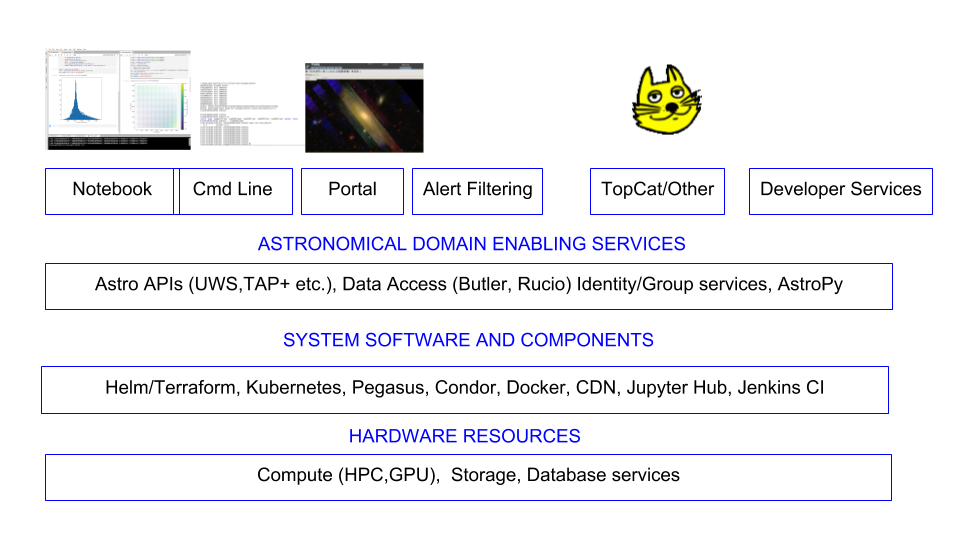
\includegraphics[width=0.45\textwidth]{CI-LSST}
\caption{Industry standard Cyber infrastructure model (left) and an astronomy instantiation of such a model (right)\label{fig:ci}}
\end{figure}

All funded funded astronomical projects with \emph{software deliverables leverage these APIs} for data access.
Of course this is not quite enough - the  \gls{API} layers must \emph{expose both data and \gls{metadata} in common
transferable and transformable formats} (e.g. \gls{CAOM}.

The astronomical community must develop \emph{data and \gls{metadata} transform services}
to support these common \gls{API} layers to aid interoperation. To further aid ease of use and cut down on wasted effort
all data providers should  to subscribe to a
\emph{common federated identity service} (e.g. InCommon or
Globus Auth) that is supported by most university and research organizations. There
must also be
an authentication source for users at institutions without such means and for
citizen science efforts.

This would imply that \emph{POSIX based file access be deprecated
in software development} and only used when applications require thread safe
data access (something that is currently not possible with \gls{FITS} files).

We should furthermore  develop a pseudo-directory structure system to
integrate local and remote files into a dynamic namespace for each user and potentially
each users use-case (e.g. the Box sync interface or the \gls{FUSE} based WholeTale file system
\citep{BRINCKMAN2019854})

\section{Why we should kill the filesystem}

Users should not care and repositories should not be tied to legacy formats  and storage representations because of legacy constraints  at other repositories.
The rest of the world has already moved on,  Google, Amazon, Git, netflix etc. do not host large filesystems and and can scale because they are not limited by this antiquated formalism.


Filesystems with name spaces are very fragile at large scale. As we get larger data sets we have to trick the filesystem to not run out of Inodes, we make countless sub directories to cope with our thousands of files.
This is turn leads to countless hours spent fighting over how to organize files  the \emph{right way} in a filesystem.
Countless years have been spent fighting over data formats (\gls{FITS} vs \gls{HDF} vs \gls{CSV} vs Pandas).
If we move code then perhaps the filesystem is not organised in the same manner and the code may not work - remote access to allow caching is not always an option.

We need to foster better remote collaboration.  The laptop is the bane of file sharing.
This has changed with cloud based pseudo-file systems but require storage in a single
cloud providers infrastructure. By creating a Filesystem as a Service (\gls{FSAAS}) federated
across data and cloud providers, we will win.


This "Infrastructure as Code" \citep{morris2016infrastructure} approach lowers the bar to entry
and allows for easier adoption of more standardized services that will enable large-scale
astronomical research in ways that are well demonstrated in plant genomics (CyVerse and Galaxy), natural hazards (Designsafe), and surface water research (Hydroshare).

\section{Example Service Architecture- The Butler}
The LSST butler

\section{Library example - AstroPy}
What is needed to go beyond \gls{LSST} and AstroPy?




% Include all the relevant bib files.
% https://lsst-texmf.lsst.io/lsstdoc.html#bibliographies
\bibliographystyle{yahapj}
\bibliography{local,lsst,lsst-dm,refs_ads,refs,books}

%Make sure lsst-texmf/bin/generateAcronyms.py is in your path
\section{Acronyms used in this document}\label{sec:acronyms}
\addtocounter{table}{-1}
\begin{longtable}{|l|p{0.8\textwidth}|}\hline
\textbf{Acronym} & \textbf{Description}  \\\hline

API & Application Programming Interface \\\hline
AURA & Association of Universities for Research in Astronomy \\\hline
AWS & Amazon Web Services \\\hline
Butler & A middleware component for persisting and retrieving image datasets (raw or processed), calibration reference data, and catalogs. \\\hline
CAOM & Common Archive Observation Model \\\hline
CI & Continuous Integration \\\hline
CRUD & Create Retrieve Update and Destroy \\\hline
CSV & Comma Separated Values \\\hline
Center & An entity managed by AURA that is responsible for execution of a federally funded project \\\hline
DMTN & DM Technical Note \\\hline
Data Management & The LSST Subsystem responsible for the Data Management System (DMS), which will capture, store, catalog, and serve the LSST dataset to the scientific community and public. The DM team is responsible for the DMS architecture, applications, middleware, infrastructure, algorithms, and Observatory Network Design. DM is a distributed team working at LSST and partner institutions, with the DM Subsystem Manager located at LSST headquarters in Tucson. \\\hline
FITS & Flexible Image Transport System \\\hline
FSAAS & Filesystem as a Service \\\hline
FUSE & a user space filesystem framework \\\hline
HDF & Hierarchical Data Format \\\hline
HPC & High Performance Computing \\\hline
HTC & High Throughput Computing \\\hline
IRAF & Image Reduction and Analysis Facility \\\hline
JSON & JavaScript Object Notation \\\hline
LSST & Large Synoptic Survey Telescope \\\hline
Object & In LSST nomenclature this refers to an astronomical object, such as a star, galaxy, or other physical entity. E.g., comets, asteroids are also Objects but typically called a Moving Object or a Solar System Object (SSObject). One of the DRP data products is a table of Objects detected by LSST which can be static, or change brightness or position with time. \\\hline
POSIX & Portable Operating System Interface \\\hline
algorithm & A computational implementation of a calculation or some method of processing. \\\hline
metadata & General term for data about data, e.g., attributes of astronomical objects (e.g. images, sources, astroObjects, etc.) that are characteristics of the objects themselves, and facilitate the organization, preservation, and query of data sets. (E.g., a FITS header contains metadata). \\\hline
pipeline & A configured sequence of software tasks (Stages) to process data and generate data products. Example: Association Pipeline. \\\hline
provenance & Information about how LSST images, Sources, and Objects were created (e.g., versions of pipelines, algorithmic components, or templates) and how to recreate them. \\\hline
\end{longtable}


\end{document}
